\documentclass{jknotes}
\usepackage{joshkirklin,pgfplots}

\usepackage{xcolor}
\usepackage{wrapfig}
\usepackage{placeins}
\usepackage{cancel}
\newcommand{\VL}[1]{\mathbf{#1}}
\newcommand{\Ro}{Ro}
\newcommand{\Ek}{E}
\newcommand{\vare}{\varepsilon}
\newcommand{\sgn}{\text{sgn}}
\renewcommand{\u}{\bm{u}}

\usepackage{tikz}
\usepackage{tikz-3dplot}
\usepackage{pgfplots}
\pgfplotsset{compat = 1.3}
\usetikzlibrary{arrows}
\usetikzlibrary{calc}

\tikzset{
    partial ellipse/.style args={#1:#2:#3}{
        insert path={+ (#1:#3) arc (#1:#2:#3)}
    }
}

\begin{document}

\institution{Cambridge Part III Maths}
\title{Fluid Dynamics of Climate}
\lecturer{John Taylor \& Peter Haynes}
\notetaker{Charles Powell}
\date{Michaelmas 2020}

\maketitle
\suggestionsspiel
\tableofcontents

\lecture{12/10/20}
\section{Fluid motion in a rotating reference frame}
In a non-rotating frame, the \emph{Navier-Stokes} equations are
\begin{equation}
	\rho \frac{\diffD \bm{u}}{\diffD t} = -\nabla p - \rho \nabla \phi + \rho
	\bm{F}
	\label{ns}
\end{equation}

The body forces are assumed to be conservative with potential $\phi$, e.g.
$\phi = gz$ for gravitational force. $\bm{F}$ is the frictional force.

Consider a reference frame rotating about the $z$-axis with constant angular
velocity $\bm{\Omega}$. Axes in the inertial frame are denoted with a
subscript $_I$ and axes in the rotating frame are denoted with a subscript
$_R$.

\begin{center}
\newcommand{\TikzInnerSep}{0.33mm}

% Define new arc command
% Syntax: [draw options] (center) (initial angle:final angle:radius)
% https://tex.stackexchange.com/a/66220
\def\centerarc[#1](#2)(#3:#4:#5){%
	\draw [#1] ($(#2)+({#5*cos(#3)}, {#5*sin(#3)})$) arc (#3:#4:#5)%
}

% Redefine the rotation sequence for the tikz3d-plot to Euler-Angles:
% z-x-z with alpha-beta-gamma (psi-theta-phi)
% https://tex.stackexchange.com/q/118069/98906
\newcommand{\tdseteulerzxz}{%
	\renewcommand{\tdplotcalctransformrotmain}{%
		%
		% Determine the sin and cos of the specified angle in degrees
		% \tdplotsinandcos{sin}{cos}{theta}
		% - #1: Returns sin(#3)
		% - #2: Returns cos(#3)
		% - #3: User-specified angle theta
		\tdplotsinandcos{\sinalpha}{\cosalpha}{\tdplotalpha} 
		\tdplotsinandcos{\sinbeta}{\cosbeta}{\tdplotbeta}
		\tdplotsinandcos{\singamma}{\cosgamma}{\tdplotgamma}
		%
		% Define trigonometric abbreviations
		%
		\tdplotmult{\sasb}{\sinalpha}{\sinbeta}
		\tdplotmult{\sacb}{\sinalpha}{\cosbeta}
		\tdplotmult{\sacbsg}{\sacb}{\singamma}
		\tdplotmult{\sacbcg}{\sacb}{\cosgamma}
		\tdplotmult{\sasg}{\sinalpha}{\singamma}
		\tdplotmult{\sacg}{\sinalpha}{\cosgamma}
		%
		\tdplotmult{\sbsg}{\sinbeta}{\singamma}
		\tdplotmult{\sbcg}{\sinbeta}{\cosgamma}
		%
		\tdplotmult{\casb}{\cosalpha}{\sinbeta}
		\tdplotmult{\cacb}{\cosalpha}{\cosbeta}
		\tdplotmult{\cacbsg}{\cacb}{\singamma}
		\tdplotmult{\cacbcg}{\cacb}{\cosgamma}
		\tdplotmult{\casg}{\cosalpha}{\singamma}
		\tdplotmult{\cacg}{\cosalpha}{\cosgamma}
		%
		% Define the entries for the rotation matrix from the B-System to the I-System
		% This is A_IB = (A_BI)^T
		%
		\pgfmathsetmacro{\raaeul}{+\cacg - \sacbsg}
		\pgfmathsetmacro{\rabeul}{-\casg - \sacbcg}
		\pgfmathsetmacro{\raceul}{+\sasb}
		%
		\pgfmathsetmacro{\rbaeul}{+\sacg + \cacbsg}
		\pgfmathsetmacro{\rbbeul}{-\sasg + \cacbcg}
		\pgfmathsetmacro{\rbceul}{-\casb}
		%
		\pgfmathsetmacro{\rcaeul}{+\sbsg}
		\pgfmathsetmacro{\rcbeul}{+\sbcg}
		\pgfmathsetmacro{\rcceul}{+\cosbeta}
		%
	}
}

% Redefine the rotation sequence for the tikz3d-plot to Cardan-Angles:
% x-y-z with alpha-beta-gamma
% https://tex.stackexchange.com/q/118069/98906
\newcommand{\tdsetcardanxyz}{%
	\renewcommand{\tdplotcalctransformrotmain}{%
		%
		% Determine the sin and cos of the specified angle in degrees
		% \tdplotsinandcos{sin}{cos}{theta}
		% - #1: Returns sin(#3)
		% - #2: Returns cos(#3)
		% - #3: User-specified angle theta
		\tdplotsinandcos{\sinalpha}{\cosalpha}{\tdplotalpha} 
		\tdplotsinandcos{\sinbeta}{\cosbeta}{\tdplotbeta}
		\tdplotsinandcos{\singamma}{\cosgamma}{\tdplotgamma}
		%
		% Define trigonometric abbreviations
		%
		\tdplotmult{\sasb}{\sinalpha}{\sinbeta}
		\tdplotmult{\sasbsg}{\sasb}{\singamma}
		\tdplotmult{\sasbcg}{\sasb}{\cosgamma}
		%
		\tdplotmult{\sacb}{\sinalpha}{\cosbeta}
		\tdplotmult{\sasg}{\sinalpha}{\singamma}
		\tdplotmult{\sacg}{\sinalpha}{\cosgamma}
		%
		\tdplotmult{\casb}{\cosalpha}{\sinbeta}
		\tdplotmult{\casbsg}{\casb}{\singamma}
		\tdplotmult{\casbcg}{\casb}{\cosgamma}
		%
		\tdplotmult{\cacb}{\cosalpha}{\cosbeta}
		\tdplotmult{\casg}{\cosalpha}{\singamma}
		\tdplotmult{\cacg}{\cosalpha}{\cosgamma}
		\tdplotmult{\cbsg}{\cosbeta}{\singamma}
		\tdplotmult{\cbcg}{\cosbeta}{\cosgamma}
		%
		% Define the entries for the rotation matrix from the B-System to the I-System
		% This is A_IB = (A_BI)^T
		%
		\pgfmathsetmacro{\raaeul}{+\cbcg}
		\pgfmathsetmacro{\rabeul}{-\cbsg}
		\pgfmathsetmacro{\raceul}{+\sinbeta}
		%
		\pgfmathsetmacro{\rbaeul}{+\casg + \sasbcg}
		\pgfmathsetmacro{\rbbeul}{+\cacg - \sasbsg}
		\pgfmathsetmacro{\rbceul}{-\sacb}
		%
		\pgfmathsetmacro{\rcaeul}{+\sasg - \casbcg}
		\pgfmathsetmacro{\rcbeul}{+\sacg + \casbsg}
		\pgfmathsetmacro{\rcceul}{+\cacb}
		%
	}
}

% Plot display orientation
\tdplotsetmaincoords{70}{150}

% Rotation angles Euler
\pgfmathsetmacro{\zOneRot}{25}
\pgfmathsetmacro{\xRot}{15}
\pgfmathsetmacro{\zTwoRot}{30}

\begin{tikzpicture}[x = 1.0cm, y = 1.0cm, z = 1.0cm, scale = 2.5, tdplot_main_coords]
	\coordinate (Origin) at (0, 0, 0);
	
	% x_I
	\draw [arrows = {}-{latex}, line width = 1.0pt] (Origin) -- (1, 0, 0)%
		node[anchor = east, xshift = -1mm, inner sep = \TikzInnerSep]%
			{$\VL{x}_I$};
	% Set the FoR orientation
	\tdseteulerzxz
	\tdplotsetrotatedcoords{\zOneRot}{0}{0}
	% x_1
	\draw [tdplot_rotated_coords, arrows = {}-{latex}, line width = 1.0pt,red] (Origin) -- (1, 0, 0)%
		node[anchor = north, yshift = -1mm, inner sep = \TikzInnerSep]%
			{$\VL{x}_R$};
	%
	% y_1
	\draw [tdplot_rotated_coords, arrows = {}-{latex}, line width = 1.0pt,red] (Origin) -- (0, 1, 0)%
		node[anchor = west, xshift = +1mm, yshift = +1mm, inner sep = \TikzInnerSep]%
			{$\VL{y}_R$};
	%
	% Draw selected axes over the grid
	% y_I
	\draw [arrows = {}-{latex}, line width = 1.0pt] (Origin) -- (0, 1, 0)%
		node[anchor = north west, xshift = +1mm, inner sep = \TikzInnerSep]%
			{$\VL{y}_I$};
	%
	% z_1
	\draw [tdplot_rotated_coords, arrows = {}-{latex},red, line width = 1.0pt] (Origin) -- (0, 0, 1)%
		node[anchor = south west, xshift = +1mm, yshift = -1mm, inner sep = \TikzInnerSep]%
		{$\textcolor{black}{\VL{z}_I} \; \textcolor{black}{=} \; \textcolor{red}{\VL{z}_R}$};
	
	% Draw rotation arrow
	\centerarc[tdplot_rotated_coords, canvas is yx plane at z=0.7, arrows = {latex}-{}](0, 0)(230 : 570 : 0.15)%
		node[anchor = north west, xshift = +2mm, yshift = -3mm, inner sep = \TikzInnerSep]%
		{$\left|\symbf{\Omega}\right| = \frac{\mathrm{d}\theta}{\mathrm{d}t}$};

	\centerarc[tdplot_rotated_coords, canvas is yx plane at z=0, arrows =
	{latex}-{}](0,0)(90:90+\zOneRot:0.6) node[midway,anchor= south] {$\theta$};

\end{tikzpicture}

\end{center}

For a point with position vector $\bm{x}$ and velocity $\bm{u}_R =
\left(\frac{\diffd \bm{x}}{\diffd t}\right)_R$ in the rotating reference
frame
\begin{equation}
	\left(\frac{\diffd \bm{x}}{\diffd t}\right)_I = 
	\left(\frac{\diffd \bm{x}}{\diffd t}\right)_R + \bm{\Omega} \times \bm{x}
\end{equation}
or equivalently $\bm{u}_I = \bm{u}_R + \bm{\Omega} \times \bm{x}$. Hence the
acceleration is
\begin{equation}
	\begin{aligned}
		\left(\frac{\diffd \bm{u}}{\diffd t}\right)_I &= 
	\left(\frac{\diffd}{\diffd t}\left[ \bm{u}_R + \bm{\Omega} \times \bm{x}
			\right]\right)_R + \bm{\Omega} \times \left( \bm{u}_R +
		\bm{\Omega} \times \bm{x}\right)_R \\
		&= \left(\frac{\diffd \bm{u}_R}{\diffd t}\right)_R + 2 \bm{\Omega}
		\times \bm{u}_R + \bm{\Omega} \times \left( \bm{\Omega} \times
		\bm{x}\right)
	\end{aligned}
\end{equation}

The first term is the acceleration in the rotating frame, the second term is
the \emph{Coriolis acceleration} and the third term is the \emph{centrifugal
accelertion}. Note that we can write the centrifugal acceleration in the form
of a conservative force
\begin{equation}
	\begin{aligned}
		\bm{\Omega} \times \left( \bm{\Omega} \times \bm{x}\right) &= \nabla
	\phi_c \\
	\phi_c &= -\frac{1}{2} \left| \bm{\Omega} \times \bm{x} \right|^2
\end{aligned}
\end{equation}

Hence the Navier-Stokes equations in a rotating reference frame are
\begin{equation}
	\rho \left( \frac{\diffD \bm{u}}{\diffD t} + 2 \bm{\Omega} \times
	\bm{u}\right) = - \nabla p - \rho \nabla \left( \phi + \phi_c\right) +
	\rho \bm{F} \label{nsrot}
\end{equation}

We group the potential terms into a \emph{geopotential} $\Phi \equiv \phi +
\phi_c$. The surface of a stationary ocean or atmosphere has a constant
\emph{geopotential height} described by an oblate spheroid.

\begin{figure}
\begin{center}
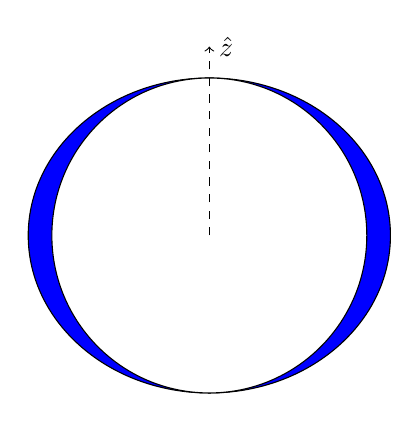
\begin{tikzpicture}
\filldraw [draw=black,fill=blue] (0,0) ellipse (2.3 and 2);
\filldraw [draw=black,fill=white] (0,0) circle (2);
\draw [dashed, ->] (0,0) -- (0,2.4) node[right] {$\hat{\bm{z}}$};
\end{tikzpicture}
\caption{Geopotential ocean surface relative to a spherical Earth.}
\label{fig:oblate}
\end{center}
\end{figure}

Imagine a spherical earth. At sea level, the polar radius is 21.4km smaller
than the equatorial radius: see figure~\ref{fig:oblate}. In reality, the
surface of the Earth is also very close to a geopotential surface. Hence
\emph{geopotential coordinates} are very useful for planetary scale motion.

\subsection{Local Cartesian coordinates}
For small motions, it is much more convenient to define \emph{local Cartesian
coordinates} (figure~\ref{fig:lcc}).
\begin{figure}
	\begin{center}
	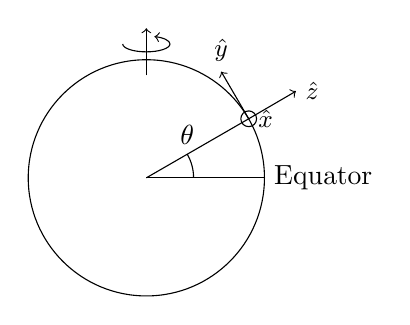
\begin{tikzpicture}
		\draw (0,0) circle (1.5);
		\draw (0,0) -- (1.5, 0) node[right] {Equator};
		\draw (0,0) -- (1.3, 0.75);
		\draw (0.6,0) arc (0:30:0.6) node[anchor = south] {$\theta$};
		\draw[->] (0,1.3) -- (0, 1.9);
		\draw[->] (0, 1.7) [partial ellipse = -180:70:0.3 and 0.1];
		\draw[->] (1.3, 0.75) -- (1.9,1.1) node[right] {\small $\hat{\bm{z}}$};
		\draw[->] (1.3, 0.75) -- (1.3 - 0.35, 0.75 + 0.6) node[above] {\small
		$\hat{\bm{y}}$};
		\draw (1.3, 0.75) circle (0.1) node[right] {\small $\hat{\bm{x}}$};
	\end{tikzpicture}
	\caption{Local Cartesian coordinates}
	\label{fig:lcc}
	\end{center}
\end{figure}

In this coordinate system $\bm{\Omega} = (0, \Omega \cos \theta, \Omega \sin
\theta)$. Hence if $\bm{u} = (u, v, w)$ then
\begin{equation}
	\begin{aligned}
		2 \bm{\Omega} \times \bm{u} &= (2\Omega w \cos \theta - 2 \Omega v \sin
		\theta, 2 \Omega u \sin \theta, -2\Omega u \cos \theta) \\
		&= (-fv + f^* w, fu - f^* u)
	\end{aligned}
\end{equation}
where $f \equiv 2 \Omega \sin \theta$ is the \emph{Coriolis parameter} and
$f^* \equiv 2 \Omega \cos \theta$.

\begin{eg}
	In Cambridge, $\theta = 52.1^{\circ} N$ so
	\begin{equation}
		\begin{aligned}
			f &= 2 \Omega \sin \theta \\
			  &= 2 \cdot \frac{2\pi}{3600 \cdot 24} \cdot 0.79 s^{-1} \\
			  &\approx 1.14 \times 10^{-4} s^{-1}
		\end{aligned}
	\end{equation}
	At mid-latitudes, $f \sim 10^{-4}$ is a good approximation.
\end{eg}

We can simplify the Coriolis acceleration expression; often $f^* w \ll f v$
and $f^* u \ll g$. Hence
\begin{equation}
	2 \bm{\Omega} \times \bm{u} \approx (-fv, fu, 0) = f \hat{\bm{z}} \times
	\bm{u}
\end{equation}

This is the \emph{traditional approximation}. This is \emph{not} always a good
approximation, particularly at intermediate scales.

\subsection{Scale analysis.}
Define characteristic scales for length $L$, time $T$, and velocity $U$.
Non-dimensional variables are denoted with a superscript star: $\bm{u}^* =
\bm{u}/U$, etc.

Using these scalings with $\bm{F} = \nu \nabla^2 \bm{u}$ we have
\begin{equation}
	\frac{U}{T} \frac{\partial \bm{u}^*}{\partial t^*} + \frac{U^2}{L}
	\bm{u}^* \cdot \nabla^* \bm{u}^* + fU \hat{\bm{z}} \times \bm{u}^* =
	-\frac{1}{\rho} \nabla \left(p + \rho \Phi\right) + \frac{\nu U}{L^2} \nabla_*^2
		\bm{u}^*
\end{equation}

Dividing through by $fU$ leaves the Coriolis acceleration term $\text{ord}(1)$ with
other terms scaled relatively.
\begin{equation}
	\frac{1}{fT} \frac{\partial \bm{u}^*}{\partial t^*} + \text{Ro}	\bm{u}^*
	\cdot \nabla^* \bm{u}^* + \hat{\bm{z}} \times \bm{u}^* =
	-\frac{1}{\rho f U} \nabla \left(p + \rho \Phi\right) + \text{E} \nabla_*^2
		\bm{u}^*
\end{equation}
where $\text{Ro} \equiv \frac{U}{fL}$ is the \emph{Rossby number} and
$\text{E} \equiv \frac{\nu}{fL^2}$ is the \emph{Ekman number}.

\begin{eg}
	For an atmospheric storm, $U \sim 10 m s^{-1}, L \sim 1000 km, f \sim
	10^{-4} s^{-1}$. Thus $\text{Ro} \sim 0.1, \text{E} \sim 10^{-13}$.
\end{eg}

\lecture{14/10/2020}
Further, if $T = L/U$, then $\text{Ro} = U/fL = 1/fT$. For small \Ro, \Ek, 
on surfaces of constant $\Phi$, $f \hat{\bm{z}} \times \bm{u} \approx
-\frac{1}{\rho}\nabla p$.  This is \emph{geostrophic balance}. In components,
we have
\begin{equation}
	\begin{aligned}
		-fv &= -\frac{1}{\rho}\frac{\partial p}{\partial x} \\
		fu &= -\frac{1}{\rho}\frac{\partial p}{\partial y}
	\end{aligned}
\end{equation}
The equations of geostrophic balance can be arranged to give the horizontal
velocity:
$\bm{u}_H$
\begin{equation}
	\bm{u}_H \equiv (u,v) = \frac{1}{\rho f} \hat{\bm{z}} \times \nabla p
\end{equation}

Horizontal velocity is perpendicular to $\nabla p$ and hence parallel to
isobars (lines of constant $p$), i.e. pressure acts like a streamfunction (see
figure~\ref{fig:isobars}).

\begin{figure}
	\centering
	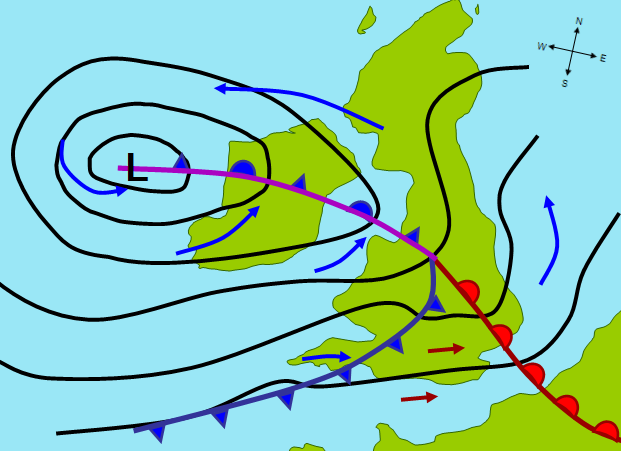
\includegraphics[width=0.4\textwidth]{isobars.png}
	\caption{Lines of constant pressure $p$ act as streamlines for the
	horizontal flow.}
	\label{fig:isobars}.
\end{figure}

In the Northern Hemisphere, air moves clockwise around high $p$ and
anticlockwise around low $p$. A \emph{cyclonic} rotation is in the same sense
as $\bm{\Omega}$, \emph{anticyclonic} in the opposite sense as $\bm{\Omega}$.

\subsection{Taylor-Proudman Theorem}
Consider an incompressible, ideal fluid in geostrophic balance (small \Ro,
\Ek)
\begin{align}
	\nabla \cdot \bm{u} &= 0\\
	2 \bm{\Omega} \times \bm{u} &= -\frac{1}{\rho}\nabla p \label{tpt}
\end{align}

Taking the curl of \eqref{tpt} we have
\begin{equation}
	\begin{aligned}
		\nabla \times \left( \bm{\Omega} \times \bm{u}\right) &= \vare_{ijk}
		\partial_j \vare_{klm} \Omega_l u_m \\
		&= \vare_{kij} \vare_{klm} \Omega_l \partial_j u_m \\
		&= \left(\delta_{il} \delta_{jm} - \delta_{im} \delta_{jl}\right)
		\Omega_l \partial_j u_m \\
		&= \Omega_i \partial_j u_j - \Omega_j \partial_j u_i
	\end{aligned}
\end{equation}

The first term is $0$ by incompressibility. Thus
\begin{equation}
	-\nabla \times \left(\bm{\Omega} \times \bm{u}\right) = \bm{\Omega} \cdot
	\nabla \bm{u} = 0
\end{equation}

For $\bm{\Omega} = (0, 0, \Omega)$, this implies $\frac{\partial w}{\partial
z} = 0$. If $w = 0$ on some horizontal surface (e.g. ground) then $w=0$
everywhere. 

Also, $u_x + v_y = 0$, i.e. horizontal velocity is non-divergent in
geostrophic balance. Fluid moves in `columns' parallel to $\bm{\Omega}$,
called \emph{Taylor columns}.

\section{Departures from geostrophy}
Consider an incompressible, rotating fluid with constant density $\rho_0$ with
angular velocity $\bm{\Omega} = (0, 0, f/2)$. Assume small ampltiude motions
(i.e. $\abs{\bm{u}}^2 \ll \abs{\bm{u}}$), i.e. neglect $\bm{u}\cdot \nabla
\bm{u}$ and $\nu \nabla^2 \bm{u}$. From \eqref{nsrot},

\begin{align}
	u_t - fv &= -\frac{p_x}{\rho_0} \label{nsrot1} \\
	v_t + fu &= -\frac{p_y}{\rho_0} \label{nsrot2}\\
	w_t &= -\frac{p_z}{\rho_0} \label{nsrot3}\\
	u_x + v_y + w_z &= 0 \label{nsrot4}
\end{align}

We will eliminate variables in favour of $p$.
\begin{equation}
	\begin{aligned}
		\nabla \cdot \left( \eqref{nsrot1} - \eqref{nsrot3}\right) &\implies
\nabla^2 p = \rho_0 f\left(v_x - u_y\right) \\
\partial_x \eqref{nsrot2} - \partial_y \eqref{nsrot1} \& \eqref{nsrot4}
&\implies (v_x-u_y)_t = fw_z \\
\end{aligned}
\end{equation}

Combining these and using \eqref{nsrot3} we have
\begin{equation}
	\nabla^2 p_{tt} + f^2 p_{zz} = 0
\end{equation}
which is a wave equation for $p$. Seek plane wave solutions with ansatz 
\begin{equation}
	p = \hat{p}e^{i\left(kx + ly + mz-\omega t\right)}
\end{equation}
and dispersion relation
\begin{equation}
	\omega^2 = \frac{f^2 m^2}{k^2+l^2+m^2} = f^2 \sin^2 \theta
\end{equation}

\begin{center}
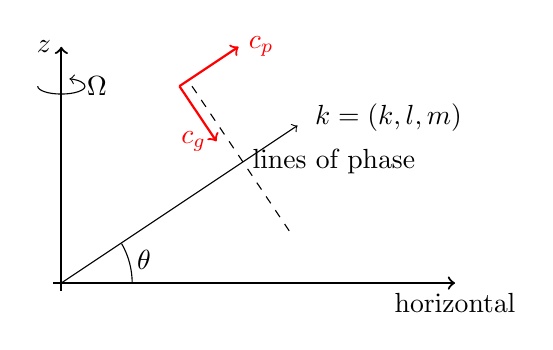
\begin{tikzpicture}
	\draw[->,thick] (-0.1,0) -- (5,0) node[below]{horizontal};
	\draw[->,thick] (0,-0.1) -- (0,3) node[left]{$z$};
	\draw[->] (0, 2.5) [partial ellipse = -180:70:0.3 and 0.1];
	\draw (0.2,2.5) node[right] {$\bm{\Omega}$};
	\draw[->] (0,0) -- (3, 2);
	\draw (3.1, 2.1) node[right] {$\bm{k} = (k, l, m)$};
	\draw (0.9,0) arc (0:30:1);
	\draw (1.05,0.3) node {$\theta$};
	\draw[dashed] (1.66, 2.5) -- (2.95,0.58) node[midway,right] {lines of phase};
	\draw[->,thick, red] (1.5, 2.5) -- (2.25, 3) node[right] {$\bm{c}_p$};
	\draw[->,thick, red] (1.5,2.5) -- (1.97, 1.8) node[left] {$\bm{c}_g$};
\end{tikzpicture}
\end{center}

This is the dispersion relation for rotating internal waves. They have phase
speed $\bm{c}_p = w/\bm{k}$ and group velocity 
\begin{equation}
	\bm{c}_g = \frac{\partial w}{\partial \bm{k}} = \pm f \frac{(-km, -lm, k^2
		+ l^2)}{\abs{\bm{k}}^{3/2}}
\end{equation}
Note that $\bm{c}_p\cdot\bm{c}_g = 0$. Also note $\abs{\omega} \le \abs{f}$.

\lecture{16/10/2020}
\subsection{Inertial (free) oscillations}
Assume $\nabla p = \bm{0}$.  The $x$ and $y$ components of geostrophic balance
\eqref{nsrot1}, \eqref{nsrot2} give
\begin{equation}
	u_{tt} + f^2 u = 0
\end{equation}
Thus $u = U \sin ft$ where $f$ is the \emph{inertial frequency}. Similarly, we
have $v = U \cos ft$. For a particle with position $(x_p, y_p)$ floating on an
ocean surface $z=0$ moving with the fluid velocity, we have
\begin{equation}
	\begin{aligned}
		\frac{\diffd x_p}{\diffd t} = u &\implies x_p = -\frac{U}{f} \cos ft +
		x_0 \\
		\frac{\diffd y_p}{\diffd t} = v &\implies y_p = -\frac{U}{f} \sin ft +
		y_0
	\end{aligned}
\end{equation}

Thus the motion of fluid particles describes describes \emph{inertial circles}
with radius $\frac{2U}{f}$.

\subsection{Ekman layer}
Look for a \emph{steady} ocean response to a constant wind stress
$\bm{\tau}_w$. Use local Cartesian coordinates and make the following assumptions:
\begin{enumerate}
	\item Steady, i.e. $\partial_t \equiv 0$
	\item Neglect horizontal variations, i.e. $\partial_x = \partial_y = 0$
	\item Neglect surface waves, i.e. $w(z=0) = 0$
	\item No flow in deep ocean, i.e. $\lim_{z \to -\infty} \bm{u} = \bm{0}$
	\item Constant density $\rho$
	\item Traditional approximation
\end{enumerate}

Continuity (incompressibility) says $u_x + v_y + w_z = 0$. Assumptions $2$ and
$3$ then imply $w = 0$ everywhere. The horizontal momentum equations are
\begin{align}
	-fv &= \nu u_{zz} \label{hmom1} \\
	fu &= \nu v_{zz} \label{hmom2}
\end{align}
Define the \emph{complex velocity} $\mathcal{V} \equiv u+iv$. Then
\begin{equation}
	\mathcal{V}_{zz} = \frac{if}{\nu} \mathcal{V} \label{compvel}
\end{equation}

Without loss of generality, assume $\bm{\tau}_w$ is aligned with the $x$-axis:
$\bm{\tau}_w = (\tau_w, 0) = (\rho \nu u_z, 0)$. Boundary conditions for
\eqref{compvel} are
\begin{equation}
	\begin{aligned}
		\mathcal{V}_z &= \left( \frac{\tau_w}{\rho \nu}, 0\right) \hspace{1em}
		\text{at} \, \, z = 0 \\
		\mathcal{V} &= (0,0) \hspace{1em} \text{as}\,\, z \to -\infty
	\end{aligned}
\end{equation}

Thus $\mathcal{V} = Ae^{(1+i)z/\delta}$ where $\delta = \sqrt{\frac{2\nu}{f}},
A = \frac{\tau_w \delta (1-i)}{2 \rho \nu}$. In terms of the velocity
components, we have
\begin{equation}
	\begin{aligned}
		u &= \frac{\tau_w}{\rho \sqrt{\nu f}} e^{z/\delta} \cos \left(
		-\frac{z}{\delta} + \frac{\pi}{4}\right) \\
		v &= -\frac{\tau_w}{\rho \sqrt{\nu f}} e^{z/\delta} \sin \left(
		-\frac{z}{\delta} + \frac{\pi}{4}\right) \\
	\end{aligned}
\end{equation}

A top view of the ocean shows an \emph{Ekman spiral}: see
figure~\ref{fig:ekman}.
\begin{figure}
	\centering
	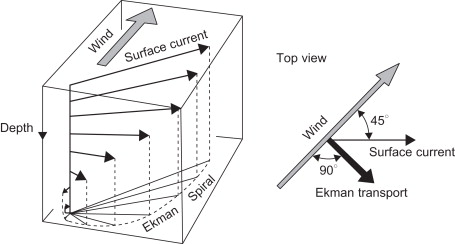
\includegraphics[width=0.5\textwidth]{ekman_spiral.jpg}
	\caption{Ekman spiral.}
	\label{fig:ekman}
\end{figure}

\subsection{Ekman transport}
Integrate the horizontal momentum equations \eqref{hmom1},\eqref{hmom2} to the
base of the Ekman layer where $\nu \bm{u}_z \approx 0$ at $z=-h$. Since $\nu
\bm{u}_z (z=0) = (\tau_w/\rho, 0)$, the \emph{Ekman transport} $\bm{U}_T$ is
\begin{equation}
	\begin{aligned}
		U_T &\equiv \int_{-h}^0 u \, \diffd z = 0 \\
		V_T &\equiv \int_{-h}^0 v \, \diffd z = -\frac{\tau_w}{\rho f}
	\end{aligned}
\end{equation}

This is the net transport of fluid in the Ekman layer and is oriented
$90^{\circ}$ to the right of the applied wind shear stress (in the Northern
Hemisphere).

\subsection{Ekman pumping}
Consider a wind stress $\tau_w(y)$ that varies over large scales. Then from
incompressibility
\begin{equation}
	\int_{-h}^0 w_z \, \diffd z = -\int_{-h}^0 u_x \, \diffd z - \int_{-h}^0
	v_y \, \diffd z
\end{equation}

Thus for $h$ constant, 
\begin{equation}-w(z=-h) = -\frac{\partial V_T}{\partial y} =
\frac{\partial}{\partial y}\left( \frac{\tau_w}{\rho f}\right)
\end{equation}

In general we have
\begin{equation}
	w(z=-h) = \hat{\bm{z}} \cdot \nabla \times \frac{\bm{\tau}_w}{\rho f}
\end{equation}

\lecture{19/10/20}
\section{Rotating shallow water equations}
Consider a thin layer of fluid with constant density $\rho$. Define
characteristic scales
\begin{itemize}
	\item length $L = \text{horiz.}, H = \text{vert.}$
	\item velocity $U$
	\item time $T$
	\item pressure $P$
\end{itemize}
such that $\partial_x, \partial_y \sim \frac{1}{L}, \partial_z \sim
\frac{1}{H}$. Define the \emph{aspect ratio} $\delta \equiv H/L$. We will
assume $\delta \ll 1$. From continuity (incompressibility) we have
\begin{equation}
	\begin{aligned}
		\frac{\partial w}{\partial z} &= -\frac{\partial u}{\partial x} -
		\frac{\partial v}{\partial y}  \\
		\implies \frac{w}{H} &= \mathcal{O}(U/L) \\
		\implies w &= \mathcal{O}(\delta U)
	\end{aligned}
\end{equation}

Using the traditional approximation and assuming the fluid is inviscid, the
$x$-momentum equation
\begin{align}
	&\frac{\partial u}{\partial t} &&+ u \frac{\partial u}{\partial x} &&+v
	\frac{\partial u}{\partial y} &&+ w\frac{\partial u}{\partial z} &&- fv &&=
						&&-\frac{1}{\rho} \frac{\partial p}{\partial x}
	\label{eq:swxmom}\\
	\text{scaling:}\hspace{1em} &\frac{U}{T} &&\frac{U^2}{L} && \frac{U^2}{L}
					&&\frac{wU}{H} &&fU &&= &&\frac{P}{\rho L}
\end{align}

Thus if $p_x$ appears at leading order then
\begin{equation}
	P \sim \rho U \max(L/T, U, fL)
\end{equation}

Similarly the $z$-momentum equation and its scalings are
\begin{align}
	&\frac{\partial w}{\partial t} &&+ u \frac{\partial w}{\partial x} &&+v
	\frac{\partial w}{\partial y} &&+ w\frac{\partial w}{\partial z} &&=
						&&-\frac{1}{\rho} \frac{\partial p}{\partial x} - g
	\label{eq:swzmom} \\
	\text{scaling:}\hspace{1em} &\frac{w}{T} &&\frac{Uw}{L} && \frac{Uw}{L}
					&&\frac{w^2}{H} &&= &&\frac{P}{\rho H}
\end{align}

Hence $\frac{\diffD w}{\diffD t} \sim \max(\frac{w}{T}, \frac{Uw}{L})$. Comparing with the
pressure term, we have
\begin{align}
	\frac{\frac{\diffD w}{\diffD t}}{\frac{1}{\rho}\frac{\partial p}{\partial
		z}} &\sim \frac{\max(\frac{w}{T},
		\frac{Uw}{L})}{\frac{U}{H}\max(\frac{L}{T}, \frac{U}{L}, f)}\\
		&\sim \delta^2
		\frac{\max(\frac{1}{T},\frac{U}{L})}{\max(\frac{1}{T},\frac{U}{L},f)}
\end{align}

Therefore to $\mathcal{O}(\delta^2)$ we have \emph{hydrostatic balance}. To
this order, \eqref{eq:swzmom} becomes
\begin{equation}
	\frac{\partial p}{\partial z} - \rho g \implies p = \rho g (\eta - z)
\end{equation}
assuming $p = 0$ at $z = \eta(x,y,t)$. Similarly, we have $\frac{1}{\rho} p_x
= g \eta_x$ and $\frac{1}{\rho} p_y = g \eta_y$. Hence horizontal acceleration
(i.e. the LHS of \eqref{eq:swxmom}) is independent of $z$. Motivated by this,
we \emph{assume} that horizontal velocity is also independent of $z$. For $\Ro
\ll 1$, this follows from the Tayor-Proudman theorem.

Re-writing \eqref{eq:swxmom} with these results we have
\begin{align}
	u_t + u u_x + v u_y -fv &= -g \eta_x \label{eq:swx}\\
	v_t + u v_x + v v_y + fu &= -g \eta_y \label{eq:swy}
\end{align}
since $u_z = v_z = 0$ by assumption. Integrating the continuity equation gives
\begin{equation}
	w = -z(u_x + v_y) + A(x,y,t)
\end{equation}
where $A$ is to be determined by the boundary conditions. Requiring no normal
flow at $z = -H_0 + h_b$ is imposed by $\bm{u}\cdot\hat{\bm{n}} = 0$ where
$\bm{n} = \nabla(z-h_b)$. Thus
\begin{equation}
	-u\frac{\partial h_b}{\partial x} -v \frac{\partial h_b}{\partial y} + w = 0
\end{equation}

Hence
\begin{equation}
	A(x,y,t) = u \frac{\partial h_b}{\partial x} + v \frac{\partial
	h_b}{\partial y} + (-H_0 + h_b) (u_x+v_y)
\end{equation}

The kinematic boundary condition at $z = \eta$ is $\frac{\diffD \eta}{\diffD
t} = w$ which may be written as
\begin{equation}
	\eta_t + u \eta_x + v \eta_y - w = 0
\end{equation}
where $w = -\eta(u_x+v_y) + u \frac{\partial h_b}{\partial x} + v
\frac{\partial h_b}{\partial y} + (-H_0 + h_b)(u_x+v_y)$. Combining these
boundary conditions gives
\begin{equation}
	\eta_t + \left[ (H_0-h_b+\eta)u\right]_x + \left[ (H_0-h_b+\eta)v\right]_y
	= 0 \label{eq:swcon}
\end{equation}
If $H \equiv H_0 - h_b + \eta$ is the total depth of the fluid, then since
$H_t = \eta_t$,
\begin{equation}
	H_t + (uH)_x + (vH)_y = 0 \label{eq:swcon2}
\end{equation}
which is a statement of the conservation of volume (equivalently mass, since
$\rho$ is constant). Equations \eqref{eq:swx}, \eqref{eq:swy}, and
\eqref{eq:swcon} are the \emph{rotating shallow water} (SW) equations.

\subsection{Potential vorticity (PV)}
Denote the vertical vorticity by $\zeta = v_x - u_y$. Consider $\partial_x
\eqref{eq:swy} - \partial_y \eqref{eq:swx}$, which gives
\begin{equation}
	\zeta_t +u\zeta_x + v\zeta_y + v f_y = -(\zeta + f)(u_x+v_y)
\end{equation}
Now from conservation of volume \eqref{eq:swcon2},
\begin{equation} 
	u_x + v_y = -\frac{1}{H} \frac{\diffD H}{\diffD t}
\end{equation}
Combining these relates the material derivative of $\zeta$ and $H$ by
\begin{equation}
	\frac{\diffD \zeta}{\diffD t} + \frac{\diffD f}{\diffD t}= \frac{\zeta + f}{H} \frac{\diffD H}{\diffD
	t} \implies \frac{\diffD}{\diffD t}\left(\frac{\zeta + f}{H}\right) = 0
	\label{eq:PV}
\end{equation}

Let $q \equiv \frac{\zeta + f}{H}$, the \emph{shallow water potential
vorticity} (SWPV). SWPV is conserved following fluid motion. We call $\zeta$
the \emph{relative vorticity} and $f$ the \emph{planetary vorticity}. $\zeta$
and $f$ will change as a fluid moves to conserve SWPV (changing $f$) and
angular momentum (changing depth).

\begin{center}
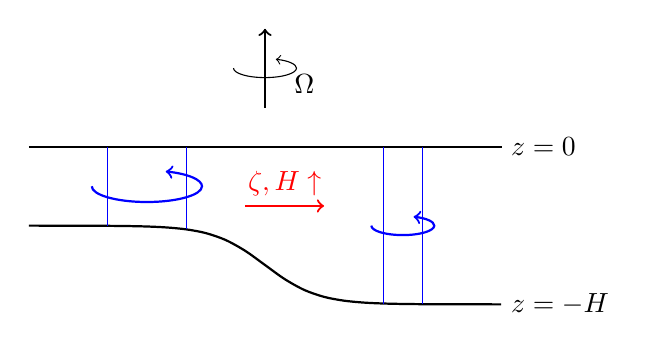
\begin{tikzpicture}
	\draw[thick,->] (0,2.5) -- (0, 3.5);
	\draw[->] (0, 3) [partial ellipse = -180:70:0.4 and 0.12];
	\draw (0.5, 2.8) node {$\bm{\Omega}$};
	\draw[thick, smooth,domain=-3:3] plot({\x}, {1/(1+exp(3*\x))});
	\draw[thick, smooth,domain=-3:3] plot({\x}, {2});
	\draw (3,2) node[right] {$z=0$};
	\draw (3,0) node[right] {$z=-H$};
	\draw[blue] (-2,0.998) -- (-2,2);
	\draw[blue] (-1,0.953) -- (-1,2);
	\draw[blue] (1.5,0.011) -- (1.5, 2);
	\draw[blue] (2,0.002) -- (2,2);
	\draw[thick,blue,->] (1.75, 1) [partial ellipse = -180:70:0.4 and 0.12];
	\draw[thick, blue,->] (-1.5, 1.5) [partial ellipse = -180:70:0.7 and 0.2];
	\draw[red, thick, ->] (-0.25,1.25) -- (0.75, 1.25) node[midway,above]
		{$\zeta, H \uparrow$};
\end{tikzpicture}
\qquad
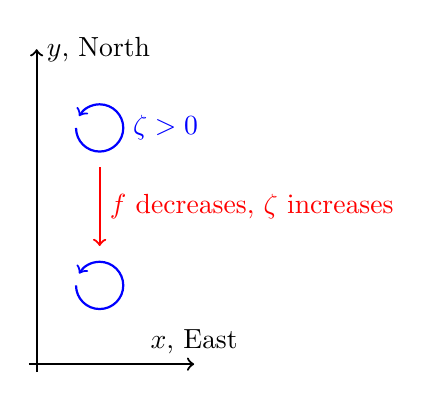
\begin{tikzpicture}
	\draw[thick,->] (-0.1,0) -- (2, 0) node[above] {$x$, East};
	\draw[thick,->] (0,-0.1) -- (0, 4) node[right] {$y$, North};
	\draw[thick,blue,->] (0.5, 3) arc(-180:150:0.3);
	\draw[thick,blue,->] (0.5, 1) arc(-180:150:0.3);
	\draw[thick,red,->] (0.8, 2.5) -- (0.8, 1.5) node[midway,right] {$f$
		decreases, $\zeta$ increases};
	\draw[blue] (1.1, 3) node[right] {$\zeta > 0$};
\end{tikzpicture}
\end{center}

\lecture{21/10/20}
\section{Small amplitude motions in rotating SW}
Consider a stationary fluid with depth $H_s(x,y) = H_0 - h_b$. The fluid
surface is then perturbed by $\eta(x,y,t)$ where $\eta \ll H_s$. The total
depth is $H(x,y,t) = H_s + \eta$. For $\abs{\bm{u}}^2 \ll \abs{\bm{u}}$,
linearise the shallow water equations:
\begin{align}
	u_t - fv &= -g \eta_x \label{swlin1} \\
	v_t + fu &= -g \eta_y \label{swlin2}\\
	\eta_t + (uH_s)_x + (vH_s)_y &= 0 \label{swlin3}
\end{align}

Assuming $f$ is constant, we have from $\partial_x \eqref{swlin1} + \partial_y
\eqref{swlin2}$ and $\partial_y \eqref{swlin1} - \partial_x \eqref{swlin2}$:
\begin{equation}
	\partial_t \left[ \left(\partial_t^2 + f^2\right) \eta - \nabla
		\cdot\left(gH_s \nabla \eta \right)\right] - fg J(H_s, \eta) = 0
		\label{swlin6}
\end{equation}
where the Jacobian $J(a,b) = a_x b_y - a_y b_x$. For the velocity components
we have
\begin{align}
	\left( \partial_t^2 + f^2\right)u &= -g\left( \eta_{xt} + f\eta_y\right)
	\label{swlin4}\\
	\left( \partial_t^2 + f^2\right)v &= -g\left( \eta_{yt} +
	f\eta_x\right)\label{swlin5}
\end{align}

\subsection{Steady flows}
We now assume $\partial_t = 0$. From \eqref{swlin4}, \eqref{swlin5},
\begin{equation}
	u = -\frac{g}{f}\eta_y, \hspace{2em} v = \frac{g}{f}\eta_x
\end{equation}
This is \emph{shallow water geostrophic balance}: the surface displacement
$\eta$ acts as a streamfunction. Applying the steady assumption to
\eqref{swlin6} gives $J(H_s, \eta) = 0$ which implies $\eta = \eta(H_s(x,y))$.
Hence linearised steady geostrophic flow in shallow water follows contours of
constant depth.  Steady PV conservation follows from \eqref{eq:PV} with
$\partial_t = 0$ and assuming $\zeta \ll f$
\begin{equation}
	\bm{u} \cdot \nabla \frac{f}{H_s} = 0
\end{equation}
Thus when $f$ varies, the flow follows contours of constant $f/H_s$.

\subsection{Waves in an unbounded domain}
Assume $H_s$ is constant. From \eqref{swlin6}, we have
\begin{equation}
	\left( \partial_t^2 + f^2\right)\eta - gH_s \nabla^2 \eta = 0
\end{equation}

Seek plane wave solutions to this wave equation with ansatz $\eta = \eta_0
\exp(i(kx+ly-\omega t))$. The dispersion relation is then
\begin{equation}
	\omega^2 = f^2 + gH_s (k^2 + l^2) \label{eq:poindisp}
\end{equation}

If $f = 0$, i.e. no rotation, then the frequency is $\omega = \pm \sqrt{gH_s}
\abs{\bm{k}} = \omega_0$ and the phase speed is $\abs{c_p} =
\frac{\abs{\omega}}{\abs{\bm{k}}} = \sqrt{gH_s} = c_0$. For $f \ne 0$, we get
\emph{Poincar\'{e}} waves with
\begin{equation}
	\omega^2 > \omega_0^2, \hspace{2em} \abs{c_p} > c_0
\end{equation}
i.e. rotation increases the frequency and phase speed. Define the \emph{Rossby
deformation scale} $R_D \equiv \frac{c_0}{f}$. From \eqref{eq:poindisp},
\begin{equation}
	\frac{\omega^2}{f^2} = 1 + R^2_D \abs{\bm{k}}^2
\end{equation}

Without loss of generality, let $l = 0$, by reorienting $x$ and $y$. If $\eta
= \eta_0 \cos(kx-\omega t)$ then \eqref{swlin4}, \eqref{swlin5} imply the
fluid velocity is
\begin{align}
	u &= \frac{\omega_0 \eta_0}{k H_s} \cos(kx-\omega t) \\
	v &= \frac{f \eta_0}{k H_s}
\end{align}
Thus the motion is an ellipse, also known as a \emph{tidal ellipse}, which
reduces to intertial circles if $\omega_0 = f$:
\begin{equation}
	u^2 + \frac{\omega_0^2}{f^2} v^2 = \frac{\omega_0^2 \eta_0^2}{k^2 H_s^2}
\end{equation}
Since $\omega > f$, the fluid moves anticylonically. The Rossby deformation
scale $R_D$ is the length scale for which rotation becomes important. Consider
short and long waves:
\begin{itemize}
	\item Short waves: $\abs{\bm{k}} R_D \gg 1$. We have $\omega^2 \to g H_s
		\abs{\bm{k}}^2$ i.e. non-rotating shallow water gravity waves.
	\item Long waves: $\abs{\bm{k}}R_D \ll 1$. We have $\omega^2 \to f^2$ i.e.
		inertial waves where fluid moves in inertial circles. Gravity is not
		involved.
\end{itemize}

\lecture{23/10/20}
\section{Geostrophic adjustment}
Consider the response of rotating shallow water to an initial state \emph{not}
in geostrophic balance. Here, we consider $\eta(x,y,) = \eta_0 \sgn(x)$,
$\bm{u}(x,y,0) = \bm{0}$, so the initial PV is $0$. 


Assume $f$ is constant, the perturbation is small $\eta_0 \ll H$, the PV is
small $\zeta \ll f$, and the bottom is flat $H_s = H_0$. Linearise the shallow
water PV:
\begin{equation}
	q = \frac{f+\zeta}{H_0+\eta} = \frac{f}{H_0}\left(1+\frac{\zeta}{f} +
		\dots\right)\left(1-\frac{\eta}{H_0}+\dots\right) \approx
		\frac{f}{H_0}\left(1+\frac{\zeta}{f} - \frac{\eta}{H_0}\right)
\end{equation}

Since PV is conserved, we have
\begin{equation}
	\frac{\zeta}{f} - \frac{\eta}{H_0} = -\frac{\eta_0}{H_0} \sgn(x)
	\hspace{2em} \forall t \label{eq:PVcons}
\end{equation}

By symmetry, $\partial_y \equiv 0$ so the PV is $\zeta = v_x$. The linearised
shallow water equations in this case
\begin{align}
	u_t - fv &= -g\eta_x \\
	v_t + fu &= 0 \\
	\eta_t + H_0 u_x &= 0
\end{align}

Using these equations we have
\begin{equation}
	\zeta = v_x = \frac{u_{xt} + g\eta_{xx}}{f} = -\frac{1}{f H_0} \eta_{tt} +
	\frac{g}{f}\eta_{xx}
\end{equation}

Now conservation of potential vorticity \eqref{eq:PVcons} gives
\begin{equation}
	\eta_{tt} - c^2 \eta_{xx} + f^2 \eta = f^2 \eta_0 \sgn(x)
\end{equation}
where $c^2 \equiv g H_0$. This is a \emph{Klein-Gordon equation} where the
$f^2\eta$ term adds elasticity to the waves.

\subsection{Steady solutions}
Consider steady solutions. Owing to the step forcing, our BCs are to match
$\eta_x$ and $\eta$ at $x=0$. We find
\begin{equation}
	\eta = \eta_0 \begin{cases} 1 - e^{-x/R_d} & x > 0 \\ -1 + e^{x/R_d} & x <
	0 \end{cases} \label{eq:gasoln}
\end{equation}
where $R_d \equiv \sqrt{gH_0}/f$ is the \emph{deformation radius}. From the
equations of geotrophic balance we have the velocity components
\begin{equation}
	u = 0, \hspace{2em} v = \frac{g \eta_0}{fR_d} e^{-\abs{x}/R_d}
\end{equation}
\begin{center}
	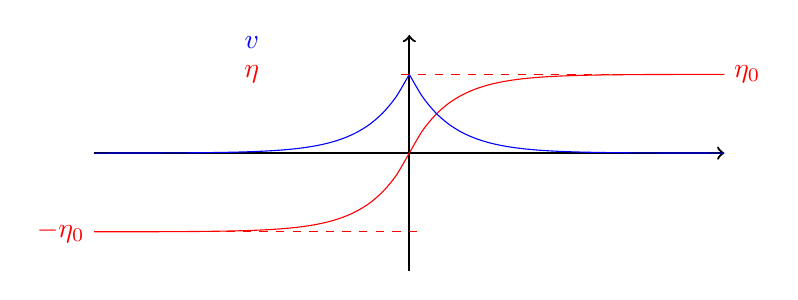
\begin{tikzpicture}
		\draw[thick,->] (-4,0) -- (4,0);
		\draw[thick,->] (0,-1.5) -- (0,1.5);
		\draw[smooth,domain=0:4,red] plot({\x},{1-exp(-2*\x)});
		\draw[smooth,domain=-4:0,red] plot({\x},{-1+exp(2*\x)});
		\draw[smooth,domain=0:4,blue] plot({\x},{exp(-2*\x)});
		\draw[smooth,domain=-4:0,blue] plot({\x},{exp(2*\x)});
		\draw[red,dashed] (-0.1,1) -- (4, 1) node[right] {$\eta_0$};
		\draw[red,dashed] (0.1,-1) -- (-4, -1) node[left] {$-\eta_0$};
		\draw[red] (-2, 1) node {$\eta$};
		\draw[blue] (-2, 1.4) node {$v$};
	\end{tikzpicture}
\end{center}

\subsection{Transients}

The steady solution \eqref{eq:gasoln} solves the geostrophic adjustment
equation, but it does not match the initial conditions. We add this particular
solution to a solution to the homogeneous equation
\begin{equation}
	\eta_{tt} - c^2 \eta_{xx} + f^2 \eta = 0
\end{equation}
with initial condition
\begin{equation}
	\eta = \eta_0 \sgn(x) - \eta_{\text{steady}} = \eta_0
	e^{-\abs{x}/R_d}\sgn(x)
\end{equation}

We seek solutions of plane wave form
\begin{equation}
	\eta = \hat{\eta} e^{i(kx-\omega t)}
\end{equation}
with $\omega^2 = f^2 + c^2 k^2$. These are Poincar\'{e} waves.

\subsection{Energetics}
The change in potential energy per unit length in the $y$ direction is
\begin{align}
	PE_{\text{initial}} - PE_{\text{final}} &= \int_{-\infty}^\infty
	\int_0^{\eta_i} \rho_0 g z \, \diffd z \, \diffd x - \int_{-\infty}^\infty
	\rho_0 g z \, \diffd z\,\diffd x \\
	&= 2\rho_0 g \left[ \int_0^\infty \frac{\eta_i^2}{2}\,\diffd x -
\int_0^\infty \frac{\eta_f^2}{2}\,\diffd x \right] \\
&= \rho_0 g \eta_0^2 \int_0^\infty \left[ 1- (1-e^{-x/R_d})^2\right] \, \diffd
x\\
&= \frac{3}{2}\rho_0 g \eta_0^2 R_d
\end{align}

The change in kinetic energy per unit length in the $y$ direction is
\begin{align}
	KE_{\text{initial}} - KE_{\text{final}} &= \int_{-\infty}^\infty
	\int_{-H}^{\eta_i} \frac{1}{2} \rho_0 v_i^2 \,\diffd z\, \diffd x -
	\int_{-\infty}^\infty \int_{-H}^{\eta_f} \frac{1}{2} \rho_0 v_f^2 \,\diffd
	z\, \diffd x \\
	&\approx 0 - \frac{1}{2}\rho_0 \int_{-\infty}^\infty H_s v^2_f \, \diffd x
	\\
	&= -\rho_0 H_s \int_0^\infty \frac{g^2 \eta_0^2}{f^2 R_d^2} e^{-2x/R_d} \,
	\diffd x \\
	&= -\rho_0 \frac{R_d^2 g \eta_0^2}{R_d^2}\cdot -\frac{R_d}{2} \cdot \left[
e^{-2x/R_d} \right]_0^\infty \\
&= -\rho_0 g \eta_0^2 \frac{R_d}{2}
\end{align}
Only $\frac{1}{3}$ of the potential energy released is converted into kinetic
energy of the geostrophic flow. The remainder is radiated away by Poincar\'{e}
waves.

\lecture{26/10/20}
\section{Quasi-geostrophic equations}
Large scale motions in the ocean and atmosphere are associated with small
Rossby number $\Ro \equiv \frac{U}{fL} \ll 1$. In this limit, the rotating
shallow water equations are approximated by the SW quasi-geostrophic (SW QG)
equation. Start from the SW PV equation:
\begin{equation}
	\frac{\diffD}{\diffD t}\left(\frac{\zeta + f}{H}\right) =
	0\label{eq:PVcons2}
\end{equation}

\paragraph{Assumption 1: $\Ro \ll 1$}
Assuming a small Rossby number implies the flow is close to geostrophic
balance with
\begin{equation}
	f \hat{\bm{k}} \cross \bm{u} \approx -g \nabla \eta
\end{equation}
where $\hat{\bm{k}}$ is the vertical unit vector. Define the \emph{geostrophic
streamfunction} $\psi \equiv \frac{g \eta}{f}$. In terms of this
streamfunction we have
\begin{align}
	\bm{u} &\approx - \nabla \times (\psi \hat{\bm{k}}) \\
	\zeta &= (\nabla \times \bm{u})\hat{\bm{k}} \approx \nabla^2 \psi
\end{align}

\paragraph{Assumption 2: small changes in $f$}
Recall the Coriolis parameter $f = 2 \Omega \sin \theta$ where $\theta$ is
latitude. Expand in a Taylor series about $\theta = \theta_0$ to get
\begin{equation}
	f = f_0 + y \frac{\diffd f}{\diffd y}\vert_{\theta_0} + \dots \approx f_0
	+ \beta y
\end{equation}
where $y$ is in the direction of local North, $f_0 = 2\Omega \sin \theta_0$
and $\beta$ is defined as
\begin{equation}
	\beta = \frac{1}{R} \frac{\diffd f}{\diffd \theta}\vert_{\theta_0} =
\frac{2\Omega}{R} \cos \theta_0\end{equation}
with $R$ the radius of Earth. For characteristic length scale $L$, assume
$\frac{\beta L}{f_0} \ll 1$. This is the \emph{$\beta$-plane approximation}.

\paragraph{Assumption 3: small changes in fluid height.}
This is consistent with small Rossby number: from geostrophic balance, we know
$\eta \sim \frac{f UL}{g}$ and $\frac{\eta}{H_0} \sim \frac{fUL}{gH_0} =
\frac{U}{fL} \frac{L^2}{R_D^2}$. Therefore $\eta/H_0 \ll 1$ if $\Ro \ll
\frac{R^2_D}{L^2}$. For $L \sim R_D$, $\Ro \ll 1$ implies $\eta/H_0 \ll 1$.
Further, we assume $h_b/H_0 \ll 1$. 

\paragraph{Quasi-geostrophic equations.} With these assumptions, SWPV becomes
\begin{align}
	\frac{\zeta + f}{H_0 - h_b + \eta} &\approx \frac{f_0}{H_0} \frac{1+
		\frac{\beta y}{f_0} + \frac{\zeta}{f_0}}{1 - \frac{h_b}{H_0} +
	\frac{\eta}{H_0}} \\
	&\approx \frac{f_0}{H_0} \left(1+\frac{\beta y}{f_0} + \frac{\nabla^2
\psi}{f_0} + \frac{h_b}{H_0} - \frac{f_0 \psi}{g H_0}\right) \\
&= \frac{f_0}{H_0} P_g
\end{align}
where $P_g$ is the \emph{quasi-geostrophic potential vorticity} and $\zeta =
\nabla^2 \psi, \eta = \frac{f_0 \psi}{g}$. Hence from SWPV conservation
\eqref{eq:PVcons2},
\begin{equation}
	\frac{\partial P_g}{\partial t} + \bm{u} \cdot \nabla P_g \approx 0
\end{equation}

Using $\bm{u} \approx - \nabla \times (\psi \hat{\bm{k}})$, $\bm{u} = -\psi_y,
v = \psi_x$ so
\begin{equation}
	\frac{\partial P_g}{\partial t} + J(\psi,P_g) \approx 0\label{eq:swqg}
\end{equation}
This is the \emph{shallow water Quasi-geostrophic} (SWQG) equation, which is
one equaiton for one unknown $\psi$, as opposed to SWPV with 2 unknowns
$\zeta, \eta$.

\subsection{Waves in QG}
Assume a flat bottom $h_b = 0$. Linearise \eqref{eq:swqg} about a state of
rest (i.e. neglect terms $\mathcal{O}(\psi^2)$). Then
\begin{equation}
	\frac{\partial}{\partial t} \left( \nabla^2 \psi - \frac{f_0^2}{gH_0}
	\psi\right) + \frac{\partial \psi}{\partial x}\beta = 0
\end{equation}
Seek plane wave solutions of the form
\begin{equation}
	\psi = \psi_0 e^{i(kx + ly - \omega t)}
\end{equation}
with dispersion relation
\begin{equation}
	\omega = \frac{-k \beta}{k^2 + l^2 + R_D^{-2}}, \hspace{2em} R_D \equiv
	\frac{\sqrt{gH_0}}{f_0}
\end{equation}
This is the \emph{Rossby wave dispersion relation}. Note $\omega = 0$ (i.e. no
waves) if $\beta = 0$. Also, if $h_b = 0$ and $\beta = 0$ there are no wave
solutions unlike rotating SW. Thus the QG system `filters' out Poincar\'{e}
waves. Note that $\beta = \frac{2 \Omega}{R} \cos \theta \ge 0$, hence $c_p =
\frac{\omega}{k} \le 0$. Rossby wave speed is always directed to the
\emph{west}.

Consider the size of the dynamic terms in $P_g$, specifically the ratio of
relative vorticity to surface height
\begin{equation}
	\frac{\nabla^2 \psi}{-\frac{f_0^2 \psi}{g H_0}} \sim \frac{R_D^2}{L^2}
\end{equation}

Hence relativity vorticity dominates at scales small compared to $R_D$ whilst
surface height dominates at scales large compared to $R_D$.

\subsection{Physical interpretation of Rossby waves}
Consider $L \ll R_d$ ($L \gg R_D$)  and a small perturbation in the dominant
term for the scale, $\zeta$ ($\eta$). For $L \ll R_D$, the planetary vorticity
increases (thus $\zeta$ decreases) on the westward side, whilst the planetary
vorticity decreases (thus $\zeta$ increases) on the eastward side. Hence the
perturbation propagates westwards. For $L \gg R_D$, the planetary vorticity
increases ($\eta$ increases) on the westward size and decreases ($\eta$
decreases) on the eastward side as before. Thus the perturbation propagates
to the west also. These are Rossby waves.
\begin{center}
	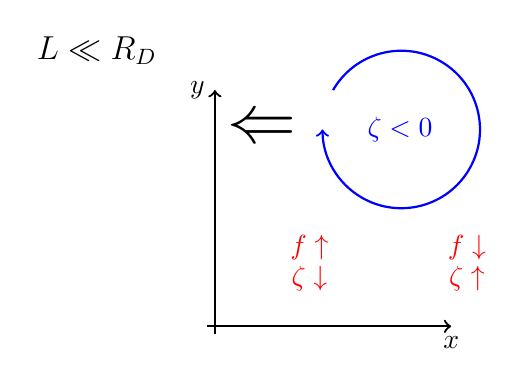
\begin{tikzpicture}
		\draw (-1.5, 3.5) node {\large $L \ll R_D$};
		\draw[thick,->] (-0.1, 0) -- (3, 0) node[below] {$x$};
		\draw[thick,->] (0, -0.1) -- (0, 3) node[left] {$y$};
		\draw[thick,blue,->] (1.5, 3) arc(150:-180:1);
		\draw[blue] (2.35, 2.5) node {$\zeta < 0$};
		\draw[red] (1.2, 1) node {$f \uparrow$};
		\draw[red] (1.2, 0.6) node {$\zeta \downarrow$};
		\draw[red] (3.2, 1) node {$f \downarrow$};
		\draw[red] (3.2, 0.6) node {$\zeta \uparrow$};
		\draw[thick] (0.6, 2.5) node {\Huge$\Leftarrow$};
	\end{tikzpicture}
	\qquad
	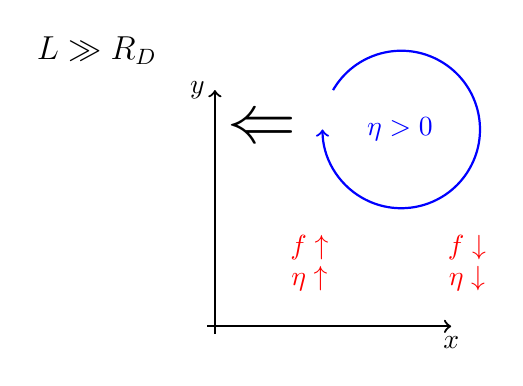
\begin{tikzpicture}
		\draw (-1.5, 3.5) node {\large $L \gg R_D$};
		\draw[thick,->] (-0.1, 0) -- (3, 0) node[below] {$x$};
		\draw[thick,->] (0, -0.1) -- (0, 3) node[left] {$y$};
		\draw[thick,blue,->] (1.5, 3) arc(150:-180:1);
		\draw[blue] (2.35, 2.5) node {$\eta > 0$};
		\draw[red] (1.2, 1) node {$f \uparrow$};
		\draw[red] (1.2, 0.6) node {$\eta \uparrow$};
		\draw[red] (3.2, 1) node {$f \downarrow$};
		\draw[red] (3.2, 0.6) node {$\eta \downarrow$};
		\draw[thick] (0.6, 2.5) node {\Huge$\Leftarrow$};
	\end{tikzpicture}
\end{center}

\section{Large scale ocean circulation}
\subsection{Sverdrup flow}
Seek steady solutions for rotating shallow water driven by a wind stress
$\bm{\tau}_w$. We have
\begin{align}
	\frac{\diffD \u}{\diffD t} + f \hat{\bm{k}}\times\u &= -g \nabla \eta +
	\frac{\bm{\tau}_w}{\rho H} \label{eq:lsoc1} \\
	H_t + \nabla \cdot (\u H) &= 0 \label{eq:lsoc2}
\end{align}

Consider $\nabla \times \eqref{eq:lsoc1} \cdot \hat{\bm{k}}$ and
\eqref{eq:lsoc2} which implies modified PV conservation
\begin{equation}
	\frac{\diffD}{\diffD t} \left( \frac{\zeta + f}{H}\right) = \frac{1}{H}
	\nabla \times \left( \frac{\bm{\tau}_w}{\rho H} \right) \cdot
	\hat{\bm{k}} \label{eq:lsocPV}
\end{equation}

Thus we see frictional forcing modifies PV conservation. Assuming $H$ is
constant, $\zeta \ll f$ ($\Ro \ll 1$), and using the $\beta$-plane
approximation $f = f_0 + \beta y$, \eqref{eq:lsocPV} becomes
\begin{equation}
	\beta v = \frac{1}{\rho H} \left(\nabla \times \bm{\tau}_w\right) \cdot
	\hat{\bm{k}}\label{eq:sb}
\end{equation}
This is called \emph{Sverdrup balance}. Physically, the North/South advection
of planetary vorticity $\bm{u}\cdot\nabla f$ balances the vorticity input by
wind.

\subsection{Western boundary currents}
Consider steady circulation in a rectangular basin, driven by a wind stress
curl
\begin{equation}
	w(y) = \frac{\left(\nabla \times \bm{\tau}_w\right)\cdot\hat{\bm{k}}}{\rho
	H} \label{eq:wbc1}
\end{equation}

\begin{center}
	\begin{tikzpicture}[scale=1.5]
		\draw (0,0) -- (5,0) -- (5,3) -- (0, 3) -- (0,0);
		\draw[thick,->] (0,0) -- (0, 1) node[left] {$y$};
		\draw[thick,->] (0,0) -- (1, 0) node[below] {$x$};
		\draw[thick, red, ->] (2, 2.8) -- (3, 2.8);
		\draw[thick, red, ->] (2, 2.7) -- (3, 2.7);
		\draw[red] (2.5, 2.55) node {westerlies};
		\draw[thick, red, <-] (2, 0.2) -- (3, 0.2);
		\draw[thick, red, <-] (2, 0.3) -- (3, 0.3);
		\draw[red] (2.5, 0.45) node {trade winds};
		\draw[thick,->] (6,0) -- (8,0) node[right] {$w(y)$};
		\draw[smooth,red] plot[domain=0:3,variable=\y] ({7-(9/8)+0.5*(\y-1.5)*(\y-1.5)},{\y});
		\draw[thick,->] (7,0) -- (7, 3.5) node[right] {$y$};
		\draw[blue,->] (2, 1.7) -- (2, 1.3);
		\draw[blue,->] (2.5, 1.7) -- (2.5, 1.3);
		\draw[blue,->] (3, 1.7) -- (3, 1.3);
		\draw[blue,->] (1.5, 1.2) arc(0:-180:0.5);
		\draw[blue,->] (3.5, 1.2) arc(-180:0:0.5);
		\draw[blue] (1,1.2) node {?};
		\draw[blue] (4,1.2) node {?};
	\end{tikzpicture}
\end{center}

From \eqref{eq:sb}, $w < 0 \implies v < 0$. Recall $\u = -\nabla \times \psi
\hat{\bm{k}}$. Boundary conditions are no normal flow at the boundaries, i.e.
$\psi$ is constant. Sverdrup balance \eqref{eq:sb} $\beta \psi_x = w(y)$ gives
\begin{equation}
	\psi = \frac{xw(y)}{\beta} + G(y)
\end{equation}
for some arbitary function $G(y)$. This presents a problem: we cannot meet the
boundary conditions at both $x=0$ and $x=L$. Hence we need extra terms and
boundary layers. Following Musk, we include horizontal friction in
\eqref{eq:lsoc1}:
\begin{equation}
	\frac{\diffD \u}{\diffD t} + f \hat{\bm{k}}\times\u = -g \nabla \eta +
	\frac{\bm{\tau}_w}{\rho H} + \nu \nabla^2 \u \label{eq:wbc2}
\end{equation}
Note here we are using the horizontal gradient $\nabla \equiv (\partial_x,
\partial_y)$. Consider $\nabla \times \eqref{eq:wbc2} \cdot \hat{\bm{k}}$ with
$\zeta \ll f$. Then
\begin{equation}
	\beta \psi_x = w(y) + \nu \nabla^4 \psi\label{eq:wbcODE}
\end{equation}
The PDE is now fourth order, so we need four boundary conditions.

\begin{center}
	\begin{tikzpicture}[scale=2]
		\draw (0,0) -- (5,0) -- (5,3) -- (0, 3) -- (0,0);
		\draw[thick,->] (0,0) -- (0, 1) node[left] {$y$};
		\draw[thick,->] (0,0) -- (1, 0) node[below] {$x$};
		\draw[dashed,blue] (0.8,0) -- (0.8, 3);
		\draw[dashed,blue] (4.2,0) -- (4.2, 3);
		\draw (2.5, 1.5) node {Interior $\psi = \psi_I$};
		\draw (0.4, 1.5) node {\small Region I};
		\draw (4.6, 1.5) node {\small Region II};
		\draw (-0.5, 1.6) node {$\psi = 0$};
		\draw (-0.5, 1.4) node {$\psi_x = 0$};
		\draw (5.5, 1.6) node {$\psi = 0$};
		\draw (5.5, 1.4) node {$\psi_x = 0$};
		\draw (2.5, 3.2) node {$\psi=0, \psi_y = 0$};
		\draw (2.5, -0.2) node {$\psi=0, \psi_y = 0$};
	\end{tikzpicture}
\end{center}

In region I we have $\psi \approx \psi_I + \psi^{(1)}$ and in region II we
have $\psi \approx \psi_I + \psi^{(2)}$. The full solution is $\psi = \psi_I +
\psi^{(1)} + \psi^{(2)}$ with interior flow $\psi_I = x\frac{w(y)}{\beta} +
G(y)$.

\lecture{30/10/20}
\paragraph{Region I.} Let $\varepsilon = \nu$ with $\vare \ll 1$. Define a
rescaled coordinate $\tilde{x} \equiv \frac{x}{\vare^a}$ with $\partial_x =
\vare^{-a}\partial_{\tilde{x}}$. Note: if $a > 0$ then $\partial_x \gg
\partial_y$. This is the \emph{method of undetermined coefficients}. From the
PDE \eqref{eq:wbcODE} for $\psi$ we have
\begin{equation}
	\cancel{\beta \psi_x^I} + \beta \vare^{-a} \tilde{\psi}_{\tilde{x}}^{(1)}
	= \vare^{1-4a} \tilde{\psi}^{(1)}_{\tilde{x}\tilde{x}\tilde{x}\tilde{x}}
	+ \cancel{w} 
\end{equation}
Matching exponents, we have $a = \frac{1}{3}$. Hence 
\begin{equation}
	\beta \tilde{\psi}_{\tilde{x}}^{(1)} =
	\tilde{\psi}^{(1)}_{\tilde{x}\tilde{x}\tilde{x}\tilde{x}}\label{eq:wbcODE2}
\end{equation}

Seek solutions of the form $\tilde{\psi} = \tilde{\psi}_0 e^{r\tilde{x}}$.
Then $r^4 - \beta r = 0$ so $r =0, \beta^{1/3}, -\frac{1}{2}\beta^{1/3} \pm
i\frac{\sqrt{3}}{2}\beta^{1/3}$. The general solution is therefore
\begin{equation}
	\tilde{\psi}^{(1)} = A(y) + B(y)e^{\beta^{1/3} \tilde{x}} +
	C(y)e^{-\beta^{1/3}\frac{\tilde{x}}{2}}e^{i\frac{\sqrt{3}}{2}\beta^{1/3}\tilde{x}}
	+ D(y)e^{-\beta^{1/3}\frac{\tilde{x}}{2}}e^{-i\frac{\sqrt{3}}{2}\beta^{1/3}\tilde{x}}
\end{equation}

In order for the interior and boundary layer flows to match asymptotically, we
apply the \emph{matching condition} $\lim_{\tilde{x} \to \infty}
\tilde{\psi}^{(1)} = 0$. Thus $A(y) = B(y) = 0$. For convenience we re-define
$C$ and $D$ to get
\begin{equation}
	\tilde{\psi}^{(1)} = C(y)e^{-\beta^{1/3}\frac{\tilde{x}}{2}} \cos \left(
	\frac{\sqrt{3}}{2}\beta^{1/3}\tilde{x} + D(y)\right)
\end{equation}

We now apply the boundary conditions. $\psi = 0$ at $x = 0$ gives
$\tilde{\psi}^{(1)} = -\psi^I\mid_{x=0}$. Hence
\begin{equation}
	C(y)\cos D(y) = -G(y)
\end{equation}
$\psi_x = 0$ at $x=0$ gives $\psi_x^{(1)} = -\psi_x^I\mid_{x=0}$. Hence
\begin{align}
	\vare^{-1/3}\tilde{\psi}_{\tilde{x}}^{(1)} &= -\frac{w(y)}{\beta} \\
	\vare^{-1/3}(-\frac{1}{2}\beta^{1/3})C(y)\cos D(y) -
	\vare^{-1/3}\frac{\sqrt{3}}{2} \beta^{1/3}C(y)\sin D(y) &=
	-\frac{w(y)}{\beta}
\end{align}

Since $\vare \ll 1$ and can be taken arbitrarily small, we require
\begin{align}
	-\frac{1}{2}\cos D(y) &= \frac{\sqrt{3}}{2}\sin D(y) \\
	\implies \tan D(y) &= -\frac{1}{\sqrt{3}} \\
	\implies D(y) &= -\frac{\pi}{6}
\end{align}

Combining the boundary conditions we also have $C(y) =
-\frac{2}{\sqrt{3}}G(y)$. Finally we have
\begin{equation}
	\tilde{\psi}^{(1)} =-\frac{2}{\sqrt{3}} G(y)e^{-\beta^{1/3}\frac{\tilde{x}}{2}} \cos \left(
	\frac{\sqrt{3}}{2}\beta^{1/3}\tilde{x} -\frac{\pi}{6}\right)
\end{equation}

\paragraph{Region II.} Here, we define a rescaled coordinate $\tilde{x} =
\frac{x-L}{\vare^{1/3}}$. The same PDE is satisfied in region II, so the
general solution is the same. Here, the matching condition is $\lim_{\tilde{x}
\to -\infty} \tilde{\psi}^{(2)} = 0$ which gives $A(y) = C(y) = D(y) = 0$, so
\begin{equation}
	\tilde{\psi}^{(2)} = B(y)e^{\beta^{1/3}\tilde{x}}
\end{equation}

We now apply the boundary conditions. $\psi_x = 0$ at $x = L$
gives
\begin{align}
	\vare^{-1/3} \tilde{\psi}^{(2)} &= -\psi_x^I \hspace{1em} \text{at}
	\hspace{1em} x=L\\
	\vare^{-1/3}\beta^{1/3}B(y) &= -\frac{w(y)}{\beta} \\
	\implies B(y) &= -\frac{\vare^{1/3}w(y)}{\beta^{4/3}}
\end{align}

To enforce $\psi = 0$ at $x = L$, note $\lim_{\vare \to 0} B(y) = 0$, so
$\tilde{\psi}^{(2)}\mid_{x=L} \to 0$ as $\vare \to 0$ so we instead require
$\psi^I\mid_{x=L} = 0$.
\begin{equation}
	\implies G(y) = -\frac{w(y) L}{\beta}
\end{equation}
Hence we have
\begin{equation}
	\tilde{\psi}^{(2)} = -\vare^{1/3} w(y)\beta^{-4/3}
	e^{\beta^{1/3}\tilde{x}}
\end{equation}

\paragraph{Full solution.} The full solution $\psi = \psi^I + \psi^{(1)} +
\psi^{(2)}$ is
\begin{align}
	\psi &= \frac{x-L}{\beta} w(y)  &&\text{interior}\\
			   &+ \frac{2w(y)L}{\sqrt{3}\beta} e^{-\beta^{1/3}
	\frac{x}{2\nu^{1/3}}} \cos\left(\frac{\sqrt{3}}{2}\beta^{1/3}\nu^{-1/3}x -
\frac{\pi}{6}\right) \hspace{.5in} &&\text{western boundary correction}\\
&- \nu^{1/3}\beta^{-4/3}w(y)e^{\beta^{1/3}\frac{x-L}{\nu^{1/3}}} 
&&\text{eastern boundary correction} \label{eq:wbc}
\end{align}

Note that the Eastern boundary correction is $\mathcal{O}(\nu^{1/3})$ whilst
the Western boundary correction is $\mathcal{O}(1)$.
\begin{figure}
	\centering
	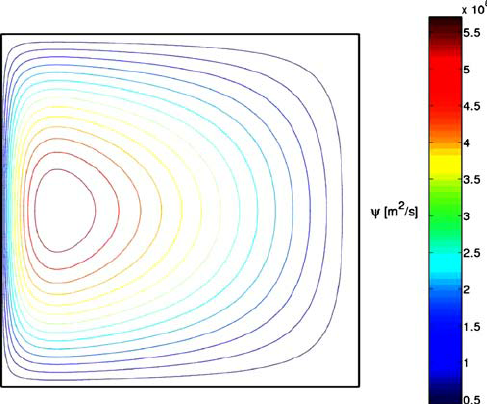
\includegraphics[width=0.4\textwidth]{wbc.png}
	\caption{Streamlines of $\psi$ demonstrating
	western boundary currents.}
\end{figure}

\paragraph{Physical explanation.} The cause of western boundary currents can
be physically explained by vorticity.  The wind stress curl $w < 0$ inputs
negative vorticity in the interior flow. The flow in the western boundary
layer inputs positive vorticity to compensate.

\begin{center}
	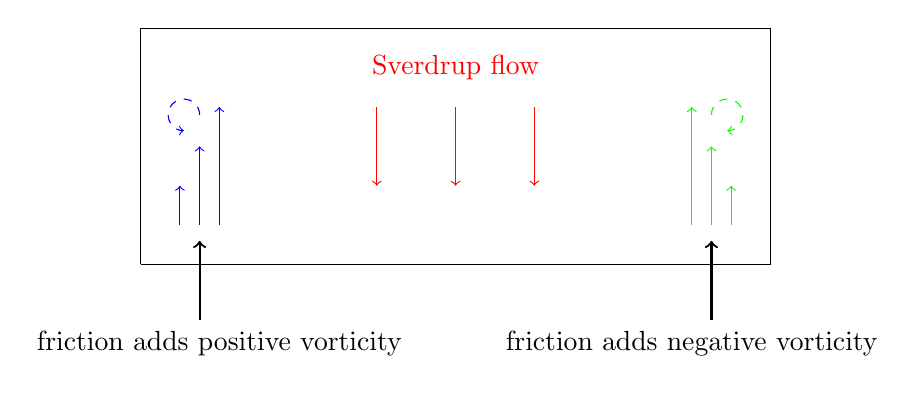
\begin{tikzpicture}
		\draw (0,0) -- (8,0) -- (8,3) -- (0,3) -- (0,0);
		\draw[red,->] (4,2) -- (4,1);
		\draw[red,->] (3,2) -- (3,1);
		\draw[red,->] (5,2) -- (5,1);
		\draw[red] (4, 2.5) node {Sverdrup flow};
		\draw[blue,->] (1,0.5) -- (1,2);
		\draw[blue,->] (0.75,0.5) -- (0.75,1.5);
		\draw[blue,->] (0.5,0.5) -- (0.5,1);
		\draw[blue,dashed,->] (0.75,1.9) arc (0:270:0.2);
		\draw[green,->] (7,0.5) -- (7,2);
		\draw[green,->] (7.25,0.5) -- (7.25,1.5);
		\draw[green,->] (7.5,0.5) -- (7.5,1);
		\draw[green,dashed,->] (7.25,1.9) arc (180:-90:0.2);
		\draw (1, -1) node {friction adds positive vorticity};
		\draw[thick,->] (0.75, -0.7) -- (0.75, 0.3);
		\draw (7, -1) node {friction adds negative vorticity};
		\draw[thick,->] (7.25, -0.7) -- (7.25, 0.3);
	\end{tikzpicture}
\end{center}

\lecture{2/11/20}
\section{Stratification}
\subsection{Boussinesq approximation}
We will consider stably stratified flow under the \emph{Boussinesq
approximation}: we assume the density $\rho$ may be split into two parts
$\rho_0$ and $\rho'$ with $\rho_0$ constant and $\rho'/\rho_0 \ll 1$. The
pressure may then also be split into two parts, $p_0(z)$, such that
$-p_0'(z) = \rho_0 g$, and the remainder $p'$. This says $p_0(z)$ is the
hydrostatic pressure and $p'$ is the excess. The vertical component of the
momentum equations may then be written
\begin{align}
	\frac{\diffD w}{\diffD t} &= -\frac{1}{\rho_0 + \rho'}\frac{\partial
		p_0}{\partial z} - \frac{1}{\rho_0 + \rho'} \frac{\partial
	p'}{\partial z} - g \\
	&= -\frac{1}{\rho_0} \frac{\partial p_0}{\partial z} + \frac{\partial
p_0}{\partial z} \left[ \frac{1}{\rho_0} - \frac{1}{\rho_0 + \rho'}\right] -
\frac{\partial p'}{\partial z} \frac{1}{\rho_0 + \rho'} - g \\
&\approx -\frac{1}{\rho_0} \frac{\partial p'}{\partial z} -
\frac{\rho'}{\rho_0} g
\end{align}
where terms including $\rho'$ are discarded unless multiplying $g$. The
\emph{Boussinesq equations} are therefore
\begin{align}
	\frac{\diffD \u}{\diffD t} + \bm{f} \times \u &= -\frac{1}{\rho_0} \nabla
	p' + \frac{\rho'}{\rho_0}\bm{g} \\
	\nabla \cdot \u &= 0 \\
	\frac{\diffD \rho'}{\diffD t} &= 0
\end{align}

These equations make clear the role of buoyancy: a light fluid parcel
experiences an upward force and a heavy fluid parcel experiences a downward
force. It is further useful to write $\rho'(x,y,z,t) = \rho_s (z) +
\tilde{\rho}(x,y,z,t)$ where $\rho_s(z)$ is a \emph{background} or
\emph{reference} density and $\tilde{\rho}$ is the \emph{disturbance density}
which is zero for fluid at rest.

The stability of the reference density state is determined by the
\emph{buoyancy frequency} or \emph{Brunt-V\"{a}is\"{a}la frequency} $N$
defined by
\begin{equation}
	N^2 = -\frac{g}{\rho_0} \frac{\diffd \rho_s}{\diffd z}
\end{equation}

\subsection{Atmosphere \& ocean stratification}
In the ocean, the buoyancy frequency $N$ is typically $10^{-2} s^{-1}$ in the
upper ocean where stratification is strong, and $5 \times 10^{-4} s^{-1}$ in
the deep ocean, where stratification is weak.

In the atmosphere, calculating $N$ needs to take account of compressibility,
because the density $\rho$ is not conserved by a fluid parcel in reversible,
dissipationless motion. The quantity that is instead conserved is the
\emph{potential temperature}
\begin{equation}
	\theta = T \left(\frac{p}{p_0}\right)^{-2/7}
\end{equation}
where $T$ is temperature. The corresponding buoyancy frequency is
\begin{equation}
	N^2 = -\frac{g}{\theta} \frac{\diffd \theta}{\diffd z}
\end{equation}

In this course we will use the Boussinesq approximation for the atmosphere and
ocean, despite issues with compressibility.

\subsection{Internal gravity waves}
We linearise about a resting state with density structure represented by the
buoyancy frequency $N$. For simplicity, background rotation is ignored for the
time being. We define the \emph{buoyancy} $\sigma = \rho' g/\rho_0$ for
convenience.

\begin{align}
	\tilde{\bm{u}}_t &= -\frac{1}{\rho_0} \nabla \tilde{p} + \tilde{\sigma}
	\hat{\bm{z}} \\
	\nabla \cdot \tilde{\u} &= 0 \\
	\tilde{\sigma} + N^2 \tilde{w} &= 0
\end{align}

where the notation $\tilde{\u}$ denotes the disturbance quantities away from a
state of rest. These can be combined into a single equation for $\tilde{w}$:
\begin{equation}
	\nabla^2 \tilde{w}_{tt} + N^2(\tilde{w}_{xx} + \tilde{w}_{yy}) = 0
\end{equation}

Assuming $N^2$ is constant, seek plane wave solutions $\tilde{w} =
\hat{w}e^{i(kx + ly + mz - \omega t)}$. This gives a dispersion relation
\begin{equation}
	\omega^2 = N^2 \frac{k^2 + l^2}{k^2 + l^2 + m^2}
\end{equation}

Note that if $N^2 > 0$ we get oscillatory motion, and if $N^2 < 0$ we get
exponentially growing disturbances. We also have $0 \le \abs{\omega} \le N$
with the lower limit achieved in the limit $k^2 + l^2 \ll m^2$. Define $\theta
= \tan^{-1}(m(k^2+l^2)^{-1/2})$, the angle a surface of constant phase makes
with the vertical. Then $\omega = \pm N \cos \theta$. Owing to
incompressibility $\nabla \cdot \u = 0$, the velocity vector is perpendicular
to $\bm{k}$. Thus $\theta$ is also the angle that fluid parcel trajectories
make with the vertical.

The fact $\abs{\omega} \le N$ implies only disturbances with a sufficiently
low frequency can propagate as waves. Localised forcing with frequency greater
than $N$ will remain localised rather than propagating. 

Further, note the group velocity is
\begin{equation}
	\bm{c}_g \equiv \frac{\partial \omega}{\partial \bm{k}} = \pm
	\frac{N}{(k^2+l^2)^{1/2} (k^2+l^2+m^2)^{3/2}} (km^2, lm^2, -m(k^2+l^2))
\end{equation}
which gives $\bm{c}_g \cdot \bm{k} = 0$, i.e. the group velocity points along
surfaces of constant phase.

\lecture{4/11/20}
\section{3D quasi-geostrophic equations}
\subsection{Basic facts about rotation \& stratification}
\begin{enumerate}
	\item Assuming the buoyancy frequency $N$ is constant and $\bm{f}$ is
		vertical, the dispersion relation for small amplitude waves is
		\begin{equation}
			\omega^2 = \frac{N^2 k^2 + f^2 m^2}{k^2 + m^2}
		\end{equation}
		where $\bm{k} = (k,l,m)$. Thus the relative strength of stratification
		vs. rotation is $N/L$ vs. $f/D$, where $L$ is the horizonal
		lengthscale and $D$ is the vertical lengthscale.
	\item Typically, $N \gg f$. In the deep ocean, $N \sim 10^{-3} s^{-1}$ and
		in the upper ocean and atmosphere $N \sim 10^{-2} s^{-1}$, whilst $f
		\sim 10^{-4} s^{-1}$.
	\item Rotation is important only if $L \gg D$, which implies vertical
		velocities are much smaller than horizontal velocities. Hence the
		\emph{hydrostatic approximation} is valid. 
	\item Given $L \gg D$, the Coriolis force may be neglected in the vertical
		momentum equation, and in the horizontal momentum equation only the
		part of the Coriolis force associateds with the horizontal velocity is
		important. This can be seen as follows: let $\bm{f} = \bm{f}_h +
		\bm{f}_v$ and $\bm{u} = \bm{u}_h + \bm{u}_v$, where $_h$ and $_v$
		denote horizontal and vertical components respectively. Then,
		\begin{equation}
			\bm{f} \times \bm{f} = \bm{f}_h \times \bm{u}_h + \bm{f}_v \times
			\bm{u}_h + \bm{f}_h \times \bm{u}_v + \cancel{\bm{f}_v \times
			\bm{u}_h} \approx \bm{f}_h \times \bm{u}_h + \bm{f}_v \times
			\bm{u}_h
		\end{equation}
		where we have assumed $\abs{\bm{u}_v} \ll \abs{\bm{u}_h}$. At low
		latitude, this assumption fails since $\bm{f}_v \ll \bm{f}_h$.
		Following the traditional approximation, only the $\bm{f}_v \times
		\bm{u}_h$ contribution is retained in the horizontal momentum
		equation. This is equivalent to replacing $\bm{f}$ with its vertical
		component only.
	\item Given the above assumptions, as well as assuming the fluid layer is
		thin compared to the radius of the Earth, we get the \emph{primitive
		equations}. 
\end{enumerate}

Further, we invoke the $\beta$-plane approximation $f = f_0 + \beta y$. The
full $3D$ Boussinesq primite equations on a $\beta$-plane are
\begin{align}
	\frac{\diffD u}{\diffD t} - (f_0+\beta y)v &= -\frac{1}{\rho_0} p'_x \\
	\frac{\diffD v}{\diffD t} + (f_0 + \beta y) u &= -\frac{1}{\rho_0} p'_y \\
	p'_z &= -\rho' g \\
	\frac{\diffD \rho'}{\diffD t} &= \\
	\nabla \cdot \bm{u} &= 0
\end{align}

This set of equations is formed of three \emph{prognostic} equations which can
be used to evolve the five dependent variables, and two instantaneous
constraints. There are strong similarities to the shallow water equations on a
$\beta$-plane: at small Rossby number, the shallow water equations have two
fast modes (e.g. Poincar\'{e} waves \& Kelvin waves for the shallow-water
equations, internal gravity waves for the primitive equations) and one slow
mode of waves which are close to geostrophic balance.

\subsection{Thermal wind equation}
When the Rossby number is small, we expect the flow to be close to geostrophic
balance, so that
\begin{align}
	-fv &= -\frac{1}{\rho_0} p'_x \\
	fu &= -\frac{1}{\rho_0} p'_y
\end{align}
Differentiating with respect to $z$ and using the hydrostatic relation, we
have the \emph{thermal wind equations}
\begin{align}
	fv_z &= -\frac{g}{\rho_0} \rho'_x \\
	fu_z &= \frac{g}{\rho_0} \rho'_y
\end{align}
Here, the density perturbation $\rho'$ can be viewed analogously to
temperature. 

\subsection{Potential vorticity}
In the shallow-water equations, the shallow-water potential vorticity was
conserved. Under the Boussinesq primite equations, instead the
\emph{Rossby-Ertal potential vorticity} P is conserved materially, where
\begin{equation}
	P = \frac{1}{\rho_0} (\bm{f} +\bm{zeta})\cdot \nabla \rho'
\end{equation}
In terms of velocities this is equivalent to
\begin{equation}
	P = \frac{1}{\rho_0} \left[ (f_v + v_x - u_y) \rho'_z + u_z \rho'_y -
		v_z
	\rho'_x\right]
\end{equation}
Note that forcing and dissipation terms are not yet included. These will give
rise to features in the $P$ field which can affect or drive the evolution of
the flow.

\subsection{3D quasi-geostrophic equations}
Following the same procedure as with the shallow-water equations, we aim to
find a prognostic equations for the slow (close to geostrophic balance) motion
from the Boussinesq primite equations on a $\beta$-plane.

We write $\rho'(x,y,z,t) = \rho_s(z) + \tilde{\rho}(x,y,z,t)$ where
$\rho_s(z)$ is in hydrostatic balance, and write $p'(x,y,z,t) = p_s(z) +
\tilde{p}(x,y,z,t)$ where each term is in hydrostatic balance with the
corresponding density term, i.e.
\begin{align}
	\frac{\diffd p_s}{\diffd z} &= -\rho_s g \\
	\frac{\partial \tilde{p}}{\partial z} &= - \tilde{\rho} g
\end{align}
The density equation $\frac{\diffD \rho'}{\diffD t} = 0$ thus becomes
\begin{equation}
	\frac{\diffD \tilde{\rho}}{\diffD t} + w \frac{\diffd \rho_s}{\diffd z} =
	0
\end{equation}

The velocity vield is divided into a part which is in geostrophic balance with
the pressure field (assuming constant $f_0$) and a remainder, the
\emph{ageostrophic velocity}:
\begin{equation}
	\bm{u} = \bm{u}_g + \bm{u}_a \hspace{2em} \text{where} \,\,\, f_0 \bm{k}
	\times \bm{u}_g = -\frac{1}{\rho_0} \nabla_h \tilde{p}
\end{equation}

Note that the vertical component of the geostrophic velocity $\bm{u}_g$ is
zero, and $\nabla \cdot \bm{u}_g = 0$. We also assume that the $y$-lengthscale
$L_y$ is sufficiently small that $\beta L_y \ll f_0$. Then if $\Ro \ll 1$, it
follows that $\abs{\bm{u}_a} \ll \abs{\bm{u}_g}$.


\end{document}
